% abstract:
% An exceptionally rare lensing configuration ?, providing a unique opportunity to explore the ISM conditions in this important but thus far unobservable(unexplored?unexploited?) regime of galaxy evolution. We propose to take advantage of the magnification of the lensed galaxy RXJ1131, a gas-rich merger with prodigious star formation rate of 120 \Msun yr\pmOne to search for OHM at intermediate-$z$, when the merger rate and ... . By combining this information with existing ?, we will ? These observations will ...


%% Suggested LaTeX template for the scientific justification
%% to be submitted as part of an NRAO observing proposal
%%
%% Version for GBT/VLA/VLBA/HSA dated 2013 July 23

\documentclass[letterpaper,11pt]{article}
\usepackage{graphics,graphicx}
\usepackage{cprotect}
\usepackage{subcaption}
\usepackage{amssymb, amsmath}
\usepackage{xspace}
\usepackage{natbibspacing, natbib}
\usepackage{aas_macros}
\usepackage{wrapfig}
\usepackage{floatrow}
\usepackage{sidecap}
%% In the graphics and graphicx packages, Postscript and eps figures
%% can be included using the \includegraphics command. The graphics
%% package is part of standard LaTeX2e and provides a basic way of
%% including a figure. The graphicx package is not standard, but
%% extends the \includegraphics command to make it more user-friendly.
%% If graphicx is not available on your system please remove it from
%% the list of included packages above.

%% Syntax:
%% In the graphics package:
%%
%% \begin{figure}
%% \includegraphics[llx,lly][urx,ury]{file}
%% \end{figure}
%%
%% where ll denotes 'lower left' and ur 'upper right' and the x and y
%% values are the coordinates of the PostScript bounding box in
%% points. There are 72 points in an inch.
%%
%% In the graphicx package:
%%
%% \begin{figure}
%% \includegraphics[key=val,key=val,...]{file}
%% \end{figure}
%%
%% where some of the useful keys are: angle, width, height,
%% keepaspectratio (='true' or 'false') and scale. Bounding box values
%% can be given as [bb=llx lly urx ury].
%%
%% In either case you have to use LaTeX figure placement commands to
%% position the figure on the page; \includegraphics will not do
%% that. Both these commands also have other options that are listed
%% in the LaTeX manual (for the graphics package) and in ``The LaTeX
%% Graphics Companion'' (for the graphicx package).

%%%%%%%%%%%%%%%%%%%%%%%%%%%
\newcommand{\Lsun}{\mbox{$L_{\odot}$}\xspace}
\newcommand{\Msun}{\mbox{$M_{\odot}$}\xspace}
\newcommand{\LIR}{\mbox{$L_{\rm IR}$}\xspace}
\newcommand{\LFIR}{\mbox{$L_{\rm FIR}$}\xspace}
\newcommand{\LOH}{$L_{\rm OH}$\xspace}
\newcommand{\rarr}{$\rightarrow$}
% \newcommand{\civ}{C{\scriptsize IV}}
% \newcommand{\heii}{He{\scriptsize II}}
\newcommand{\bco}{\mbox{CO(2-1)}\xspace}
\newcommand{\cco}{\mbox{CO(3-2)}\xspace}
\newcommand{\lohmax}{$L_{\rm OH}^{\rm max}$\xspace}
\newcommand{\lohpred}{$L_{\rm OH}^{\rm pred}$\xspace}
\newcommand{\lohlfir}{$L_{\rm OH}-L{\rm FIR}$\xspace}

% \newcommand{\Lp}[1][CO]{\mbox{$L^{\prime}_\textrm{\fontsize{8pt}{12pt}\selectfont{#1}}$}}
% \newcommand{\LpU}{\mbox{K\,\,km\,\,s$^{-1}$\,\,pc$^2$}}
\newcommand{\kms}{km\,s$^{-1}$\xspace}
\newcommand{\pmOne}{\mbox{$^{-1}$}\xspace}
\newcommand{\Fig}[1]{Fig.~\ref{fig:#1}}
\newcommand{\Eq}[1]{Equation~\ref{eq:#1}}
%
\newcommand{\E}[1]{\mbox{$\times10^{#1}$}}
\newcommand{\eq}{\,=\,}
\newcommand{\ssim}{\,$\sim$\,}
\newcommand{\pmm}{\,$\pm$\,}
%
\newcommand{\SF}{star formation\xspace}
\newcommand{\highz}{high-$z$\space}
\newcommand{\athighz}{at high redshifts\xspace}
\newcommand{\atinterz}{at intermediate redshifts\xspace}
\newcommand{\SB}{starburst\xspace}
\newcommand{\bh}{black hole\xspace}
\newcommand{\hr}{high resolution\xspace}
\newcommand{\obs}{observations\xspace}
\newcommand{\stu}{studies\xspace}
\newcommand{\galpop}{galaxy populations\xspace}
\newcommand{\qsohosts}{quasar host galaxies\xspace}
%%%%%%%%%%%%%%%%%%%%%%%%%%%

% compact bib
\citestyle{aa}
\bibliographystyle{apj_w_etal_3auth}
\usepackage{paralist}
\renewenvironment{thebibliography}[1]{%
%\section*{\refname}%
%  {\normalsize {\textbf{References:}}}
  \let\par\relax\let\newblock\relax%
  \inparaitem[{[}1{]}]}{\endinparaitem}

%%%%%%%%%%%%%%%%%%%%%%%%%%%
%%%%% Page dimensions %%%%%
%%%%%  DO NOT CHANGE  %%%%%
%%%%%%%%%%%%%%%%%%%%%%%%%%%

\setlength{\textwidth}{6.5in} \setlength{\textheight}{9in}
\setlength{\topmargin}{-0.0625in} \setlength{\oddsidemargin}{0in}
\setlength{\evensidemargin}{0in} \setlength{\headheight}{0in}
\setlength{\headsep}{0in} \setlength{\hoffset}{0in}
\setlength{\voffset}{0in}
\setlength{\parskip}{0.5em}



% added by D. Leung
\setlength{\intextsep}{10pt plus 1.0pt minus 2.0pt}
\setlength{\textfloatsep}{10pt plus 1.0pt minus2.0pt}
\setlength{\floatsep}{10pt plus 1.0pt minus 2.0pt}


%%%%%%%%%%%%%%%%%%%%%%%%%%%%%%%%%%
%%%%% Section heading format %%%%%
%%%%%%%%%%%%%%%%%%%%%%%%%%%%%%%%%%

\makeatletter
\renewcommand{\section}{\@startsection%
{section}{1}{0mm}{-0.4\baselineskip}%
{0.1\baselineskip}{\normalfont\fontsize{11}{11}\bfseries}}%
\makeatother

%%%%%%%%%%%%%%%%%%%%%%%%%%%%%
%%%%% Start of document %%%%%
%%%%%%%%%%%%%%%%%%%%%%%%%%%%%

\begin{document}
\pagestyle{plain}
\pagenumbering{arabic}


%%%%%%%%%%%%%%%%%%%%%%%%%%%%%
%%%%% Title of proposal %%%%%
%%%%%%%%%%%%%%%%%%%%%%%%%%%%%

\begin{center}
{\large{\bf{Probing OH Megamaser in a Strongly-Lensed Gas-Rich Merger at $z$\ssim0.65}}}
\end{center}
\vspace{-.8em}
\textbf{Current understanding of OH megamasers and galaxy evolution} \\
% point
% - OHM <-> ULIRGs <-> mergers <-> gas rich 
% - conditions for OHM
\indent Almost all ($>$95\%) OH ``megamasers" (OHMs) known to date are associated with 
(ultra)-luminous infrared galaxies (U)LIRGs (\LIR$>10^{11}$\,\Lsun; see \citealt[]{Lo05a} for a review), 
which are undergoing extreme bursts of star formation triggered by merger events
\citep[e.g.,][]{Sanders96a, Hopkins06b}.
Theoretically, the intense IR radiation field and the large column of molecular gas 
found in (U)LIRGs/mergers
are the required conditions for generating OHMs \citep[e.g.][]{Baan89a}.
%Since the necessary excitation of OHMs can be provided by 
%IR pumping (for pop. inversion) with large molecular column density \citep{Baan89a}, where 
%the required radiation is believed to be coming from dust absorbing starlight from 
%SB that are thought to be merger-driven (and AGN), and the high density at center easily reached in mergers.
Thus, starburst galaxies (IR-luminous) and mergers appear to be the most probable galaxy populations for hosting OHMs.

% point:
% - using OHM to trace distant merger
% - future survey using number density of OHM to constraint galaxy evolution models / merger history
% - currently no new detections beyond z>0.3, despite great efforts over the last two decades
% - our source is cheap to do, reasonable to expect OHM, we are probing deeper than previous attempts
The scaling relation of $L_{\rm OH}$$\propto L_{\rm FIR}^{2}$ 
\citep[or  $L_{\rm OH}$$\propto L_{\rm FIR}^{1.2}$ with Malmquist bias correction; \Fig{model}a; ][hereafter DG02]{Baan89a, Darling02b_LF} 
suggests that the number density of OHM is expected to increase towards $z$\ssim3,
when (U)LIRGs/mergers are more common \citep[e.g.,][]{LeFloch05a, Magnelli09a}.
OHMs have therefore been proposed as one of the most promising avenues for tracing mergers beyond the nearby universe
and for constraining the merger history of galaxies 
independent of IR luminosity function (\citealt{Briggs98a}, DG02). 
These models predict%  based on the commonly observed \LFIR$>$1\E{12}\Lsun at $z$\,$\gtrsim$\,1
that we should be able to detect OHMs out to at least $z$\ssim3 with current facilities 
(e.g. the GBT; \Fig{model}b). Yet, 
the most distant OHM host galaxy known-to-date is at $z$\eq0.265, which was 
discovered over two decades ago \citep{Baan92a}.
In addition, the null detections and unexpectedly low detection rate 
reported in the latest OHM studies (over half a decade ago) 
by \citet{Ivison06a} in a $z$\ssim4 galaxy % with an IR luminosity of \LIR$\gtrsim$1\E{14}\Lsun, 
and by \citet{Willett12a} in a sample of (U)LIRGs at $z$\,$\lesssim$\,1.5 (7\% detection rate, \Fig{model}) --- % only detected 9/121 
suggest a potential redshift evolution in the \LOH-\LFIR relation, which may hint at a different 
OHM triggering mechanism at earlier epochs that reflects the different physical conditions between
low- and high-$z$ (U)LIRGs.
The null detections in these studies also indicate also suggests that the 
classical model for OH pumping (pumped radiatively) in megamasers may not be universal (i.e., not all OHMs are unsaturated).
% only a radiative pumping mechanism for OH megamasers based on weak, unsaturated gain has been considered \citep{Henkel90a,Randell95a}.
%In these papers it was assumed that the maser cloud amplifies 
% radio emission from a source lying behind the cloud. 
However, since a purely radiative pumping mechanism is possible only at relatively low densities ($n_{\rm OH}$\ssim10$^{-4}$\,cm$^{-3}$). 
Theoretically, at relatively high OH densities, collisional processes may predominate. 
In addition, at high densities saturated amplification can be important \citep{Field94a}.
Detecting OHM beyond $z$\eq0.265 is therefore crucial to 
enable a better understanding of OHM and to 
improve existing predictions used for planning future OHM surveys with upcoming facilities 
\citep[e.g., FAST, APERTIF/WSRT, ASKAP;][]{Zhang14b}.
Here we propose to observe OH 1667 MHz line emission in the 
gravitationally-lensed starbursting galaxy merger
RXJ1131 at $z$\eq0.65 (\Fig{hst}) using the VLA's B-array configuration. 

\noindent \textbf{An ideal target --- a lensed gas-rich, starbursting merger at $z$\,$>$\,0.6}\\ 
\indent High-resolution imaging and spectroscopy in optical wavelength show that RXJ1131 is 
lensed by a foreground galaxy at $z$\ssim0.3 (\Fig{hst}; \citealt{Sluse03a}). 
By exploiting the effect of lensing magnification, 
our proposed detection experiment requires {\bf an on-source time of  % sigma scales as 1/root(t) --> t scales as 1/sigma^2
$\sim$30 times less} than otherwise needed to reach the same sensitivity. 
The unique lensing configuration of RXJ1131 has led to extensive follow-up studies spanning X-ray to radio \citep[\Fig{hst}; e.g.,][]{Claeskens06a, Sluse07a, Pooley07a, Reis14a, Leung17a}, 
making it one of the best-studied galaxies at $z$$>$0.5 and 
the only source at 0.2$<$$z$$<$1 with spatially-resolved imaging of the molecular gas distribution \citep{Leung17a}. 
The lensed nature of this target provides an excellent 
opportunity to study the innermost regions around a black hole at a cosmological distance.
In fact, X-ray studies constrained the X-ray emitting region a highly compact source of emission 
($\sim$20\,AU; constraining the optical and X-ray emitting region near the accretion disk down to pc-scale) \citep{Dai10a},
demonstrating the how much we already know about this target.
Features in the X-ray spectrum finds 
%  A fraction of this hard X-ray emission is reflected by cold gas in the accretion disk, producing an observed spectrum imprinted with the features of photoelectric absorption, fluorescent 6.4 keV Fe K$\alpha$ line emission, and a Compton backscattered reflection continuum that produces a bump in the spectrum above 10 keV (George & Fabian 1991).
 % The continuum is strongly absorbed at soft energies by a 
a neutral gas of column density $N_{\rm H}\sim$10$^{23}$ cm$^{-2}$ near the accretion disk. % w.in the X-ray emitting region
The spectrum at lower energies is heavily absorbed by neutral gas with a hydrogen column density $N_{\rm H}$.
% Soft X-ray continuum suggest the presence of a substantial amount of gas.
Our best-fit spectral energy distribution (SED) model indicates
a strong apparent far-IR luminosity of \LFIR$>$4\E{12}\,\Lsun, which corresponds to
an intense star formation rate of SFR\ssim120 \Msun yr\pmOne (lensing-corrected).
These properties together with the evidence of recent star formation (as traced by rest-frame UV \obs),
the presence of a nearby companion at $\sim$2.4\,kpc away, and a large molecular gas reservoir of $M_{\rm gas}$\,$\gtrsim$\,10$^{10}$\Msun (\Fig{hst}) 
are favourable for generating OHMs, suggesting RXJ1131 is an ideal candidate 
to search for OHM beyond the nearby universe.

In addition, the redshift of RXJ1131 has been spectroscopically confirmed with CO lines down to a precision of 
$\Delta z$\eq0.0002, indicating that the proposed OH line is redshifted to a fortuitous region 
free of RFI at the low-end of the L-band. 
This together with the high fringe rate of the B-array configuration will 
reach a sensitivity deeper than previous high-$z$ OHM searches beyond $z$$>$0.4, which were carried out 
with single-dish telescopes \citep[\Fig{model}b; e.g.][]{Darling02a, Willett12a}.


%--- added
% what can OHM help us understand the physical conditions of high-z galaxies. 
% what can't we learn from local OHM but can at high-z.
% difference between local and high-z; why care about doing OHM at high-z
The number density of IR-luminous galaxies and their molecular gas fractions and SFRs
are higher towards $z$\ssim2,
indicating a different physical conditions between low- and high-$z$ galaxies.
Such a different physical conditions can potentially be reflected in the OHM phenomenon, given that OHM are more strongly amplified in 
large column of molecular gas and the more intense IR radiation field.
Given that OHMs originate from central region, detecting OHM in high-$z$ galaxies and comparing them against those in the local, which are 
relatively more quiescent, would allow us to directly probe the physical conditions (and dynamics) in the inner few hundred pc
as galaxies evolve. {\bf justify the masing, pumping mechanism in science goals}
% foreground amplification of background radio continuum, this quadratic relationship may be expected, if the population inversion is pumped by the FIR radiation field and the radio continuum (which itself is proportional to the FIR luminosity) is being amplified by an unsaturated maser cloud
In fact, the null detection of OHM in a $z$\ssim4 galaxy with \LIR$>$1\E{13}\,\Lsun already hints at a different 
excitation mechanism that may be a result of their different physical conditions (e.g. more dense, higher optical depth \citet{Ivision06a}).

% X-ray and LOH -- why RXJ1131
Because OHMs are associated with the most luminous galaxy in the nearby universe, it is reasonable to speculate a possible connection
between OHMs and quasars, where both are driven by mergers (increasing \LFIR, and molecular gas into central region) 
since recent high-$z$ studies find evidence that AGN activity and mergers are connected (growth of SMBHs may be partly driven by 
mergers) \citep{DiMatteo05a}.
pumping and density, saturated:
 A purely radiative pumping mechanism is possible only at relatively low densities
($n_{\rm OH}$\ssim10$^{-4}$ cm$^{-3}$). At relatively high OH densities, collisional processes may predominate. In addition, at high densities
saturated amplification can be important.
While in the nearby universe (z\ssim0), OHMs appear to be unsaturated. But this may not be the case at high-$z$, where
 the physical environment is very different, more violent star formation, the ISM is more turbulent, and when there are more gas 
 available on average.
Further \obs of OHM are needed to elucidate the role of collisional processes in 
producing population inversions over the observed radiative transitions of OH.
% while locally, not all OHM are AGN hosts, suggesting the FIR radiation from the SB is the dominant pumping source, but the non-detection based on local extrapolation and such maser model may suggest a different energy source/powering mechanism/ at higher-z, where quasars are more active, and may indicate that something about AGN/radio pumping? saturated amplification?

%-------

\noindent \textbf{Science goals} \\

\indent The proposed \obs will establish the first measurement of an OHM in a {\it bona-fide} high-$z$ merger, thereby
demonstrating the feasibility of using it as a tracer of distant galaxy mergers and
testing the long-envisaged hypothesis of using the number density of OHM to constrain 
the redshift evolution of merger rate. 
Such a
high-$z$ (non-)detection will also allow us to better constrain the \LOH-\LFIR scaling relation and its redshift evolution,
and thus improve 
% current models used to predict OHM detection rate 
predictions on the detection threshold needed  
% model predictions for designing 
% when designing
% future surveys to search for 
to carry out systematic searches of high-$z$ OHMs with upcoming facilities.  
% because if we find a shallower relation, then it would mean the surveys need to go deeper to reach the same \LOH.
Since our target is a merger, 
a null detection would also indicate that the notion of 
using the OHM number density to constrain the merger history needs to be revised before designing future OHM surveys.

% --  host properties ---
% to further understand the relationship between OHM and the types of galaxies hosting them at an earlier epoch.
In addition, regardless of whether the OH line emission is detected or not, the amount of data we have already acquired 
for this potential OHM host galaxy will allow us to compare its (host) galaxy properties 
(e.g., SFR or \LFIR, \LIR, \LOH, $L_{\rm radio}$, molecular and dust content)
against those of local OHM hosts to better understand 
% the nature of OHM.
% the pumping and masing mechanism of OHM. % the condition needed for generating OHM
% the required conditions for triggering OHM at an earlier epoch.
the relationship between the maser emission and the environment of its (host) galaxy. 
{\bf  Is there some
detailed prediction that they should be found in things above a
certain SFR or merger state or something? Any more details you can
provide there would be better. But 2-3 sentences about this would be good.
LFIR, LRadio.. LOH.. 
}
% --- to better understanding the pumping and masing mechanism --
To blah... saturated maser and collisional pumping. % saturated gain mechanism
% The T/density of the masing material? 
% Maybe you could do some of that with
% certain reasonable assumptions? Similarly 2-3 sentences would be good.
% 
Because of the required condition to excite and generate OHM, and because they originate from the central few pc to few hundred pc 
in the nuclear regions of galaxies \citep{Diamond99a},
OHM is a powerful diagnostics of the physical 
conditions in the innermost regions of galaxies. 
% foreground amplification of background radio continuum, this quadratic relationship may be expected, if the population inversion is pumped by the FIR radiation field and the radio continuum (which itself is proportional to the FIR luminosity) is being amplified by an unsaturated maser cloud
Classical model of OHMs suggest that low-gain amplification (i.e., unsaturated gain) and IR pumping 
is the dominant mechanism for producing OHM. However, the null detections of OHM at $z$$>$0.3
\citep{Ivison06a, Willet12a} may suggest different pumping efficiency (\LOH/\LFIR) at high-z, due to the different physical conditions (e.g. 
optical depth is higher at high-z due to the higher LFIR). 
% 
% Since FIR radiation field can invert the OH population via the ``pumping lines'' at 35 and 53$\mu$m
% Masing can then be stimulated by 18 cm (i.e. $\sim$1.6GHz).
% With the additional constraint on the \LOH-\LFIR relation at $z$$>$0.3 provided by this experiment, we will 
% investigate the pumping efficiency at higher redshift than currently studies, %% but presumable can already do so with upper limits from Willett+12
% by comparing to local OHM hosts and as a function of \LFIR through the \LOH-\LFIR scaling relation. % (look for potential discrepancy in this relation based on nearby studies)% (already seen a discrepancy at z=3, see also Darling02b find evidence of a mixture of saturated and
% unsaturated masers). 
% For instance, a slope shallower than $<$2 %  (i.e, deviations from the quadrature) 
% would suggest that the amplification process is less efficient at higher FIR luminosity. %, where the optical depth is higher.
% Since the optical depth increases with FIR radiation field, the simple picture of low-gain amplification
% (i.e., unsaturated masing) found to be consistent with local OHMs
% will likely break down resulting in deviations from the quadratic relation 
% implying the simple picture of low-gain amplification (i.e., unsaturated masing) 
% found to be consistent with local OHMs will likely break down
% and indicate saturated masing at high redshift.
% Darling02b: find evidence of a mixture of saturated and unsaturated masers. 
% 
A non-detection would therefore still be meaningful in advancing our knowledge. 


% --- procedure
%Existing lens modeling of RXJ1131 have been carried out from rest-frame X-ray through submm, indicating BLAH component is strongly-lensed by a factor of $\mu$\ssim10. 
%Since the OHM is expected to originate from the few hundred pc from the central quasar \citep[e.g.][]{Darling07a}, thus 
%we will correct for lensing using the magnification factor based on X-ray, MIR lens model \citep{}.

With the aid of lensing and the rich multi-wavelength data 
% probing a wide range of properties 
available for this potential OHM host, RXJ1131 is an exceptional target
for obtaining a better understanding of OHM in IR-luminous galaxies beyond the nearby universe out to
a lookback time of $\sim$6 Gyr.
% The detection of a OHM at redshift higher than already known 
% may also open up/demonstrate the possibility of use OHM as a tool for studying the 
% properties (dynamics) of the molecular nuclei at high redshifts when observed at high resolution with the VLBI.
In the case of a detection, we will future carry out follow-up \obs % at higher-resolution 
with the VLBI to study the physical conditions of the nuclear molecular torus
% and to better understand the energy source and the nature of OHM at high redshift.
% ($<$ few hundred pc) 
responsible for the OH line emission, where the velocity structure of the 
currently highest-$z$ OHM already suggests a different dynamic structure 
than those at lower-$z$ \citep{Baan92a}. % . e..g IRAS F14070+0525 has a total line width of ~2400 km/s 
% OHM may be useful for studying dynamical and molecular properties of nuclei at high-z. <-- well, but APM is not detected.. so OHM may not be so reliable.
The proposed investigation will therefore serve as an
important benchmark for future studies of high-$z$ OHM out to earlier epochs,
when extremely IR-luminous sources are much more common.
%  inform future systematic searches of high-$z$ OHMs 
% Thus, a detection/non-detection at this redshift is crucial for development of this technique for future OHM studies.


%\noindent \textbf{Technical Justification}
%We estimate the required sensitivity based on the \LFIR of 4\E{12}\,\Lsun found for RXJ1131 
%together with the \LOH$\propto$\LFIR$^{1.2}$ relation reported by (DG02), and 
%the typical FWHM line width of $\sim$600\,\kms of the highest-$z$ sources ($z$$>$0.2; DG02).
%These yield a line intensity of 330 mJy\,\kms, and a peak flux density of $S_\nu$\eq0.55\,mJy.
%To secure a 5$\sigma$ detection, we therefore require $\sigma$\eq0.11\,mJy beam\pmOne over the line FWHM. 
%Since extragalactic OHMs originate from the central few hundred pc, we expect the emission to 
%remain spatially-unresolved at the B-array configuration.
%We thus require an on-source time of 4.3 hours (total time of 5.5 hours).
%% \vspace{-0.25em}

%% ------------------------------------------------------------
%% REFERENCES
%% ------------------------------------------------------------
\noindent \textbf{References}
{\fontsize{10pt}{12pt}\selectfont
    \bibliography{master_cleanup}
}
% \vspace{-1.25em}


\begin{figure}[ptbh]
\includegraphics[trim=10 305 270 0, clip, scale=0.825]{Fig/OHFIR} \hspace{-1.25em}
% \includegraphics[trim=0 400 200 0, clip, scale=0.85]{Fig/Darling02b_distribution}
%  \includegraphics[trim=0 0 0 0, clip, scale=0.625]{Fig/Willett11_distribution}\\ \vspace{1.5em}
% \includegraphics[trim=0 0 0 0, clip, scale=0.42]{Fig/Darling02_predictionf4}
\includegraphics[trim=0 -20 155 0, clip, scale=0.41]{Fig/willett12_fig1_mod.pdf}
\caption{{\bf \LOH-\LFIR correlation and existing OHMs measurements}
{\it Left}: The super-linear correlation found between \LOH and \LFIR in local studies indicates
the connection between OHM generation and IR radiation field,
and thus suggests that OHM is a powerful tool for tracing distant mergers (bright IR emitters)
and constraining the cosmic merger history (DG02).
{\it Right}: 
The highest-$z$ OHM known to date (at $z$\eq0.265) was 
detected over two decades ago \citep{Baan92a}.
3$\sigma$ sensitivity predicted to be necessary for OHM detection at different $z$, 
derived based on existing OHM detections (i.e., assuming some $\Delta v$). 
Subsequent OHM \obs yielded very low detection rate ($\sim$7\%;  black and green) \citep[figure modified from][]{Willett12a}. 
The lower than expected detection rate indicates that current prediction based on local measurements need to be revised, or that the previous 
high-z OHM survey are not sensitive enough, or that the assumption of $\Delta v$ is too small (the $z$$>$0.2 sources have wider FWHM by at least a factor of 2). 
Our proposed \obs will push beyond these sensitivity to $5\sigma$\eq0.55 mJy...
 (since RFI is better in interferometer, because higher fringe rate, increase baselines so that RFIs are decorrelated via geometric delay.)
{\bf also can reach to lower rms than previous study which are affected by RFIs.}
Here we propose to observe OH 1667 MHz line emission in the gravitationally-lensed starbursting 
galaxy merger RXJ1131 at $z$\eq0.65. 
In contrast to the \citet{Willett12a} sample, which does not include any active galactic nucleus (AGN) host 
galaxies, 
our target hosts an optically bright AGN, and thus may offer an alternate view to high-$z$ OHM hosts. 
The proposed \obs will better constrain the \LOH-\LFIR scaling relation and its redshift evolution, and thus 
improve % current models used to predict OHM detection rate 
model predictions for designing 
future surveys to search for high-$z$ OHMs with upcoming facilities.
{\bf look for discrepancy in \LOH-\LFIR between low and high-$z$ mergers/potential OHM hosts, which
 would indicate different OH excitation mechanism.} % foreground amplification of background radio continuum, this quadratic relationship may be expected, if the population inversion is pumped by the FIR radiation field and the radio continuum (which itself is proportional to the FIR luminosity) is being amplified by an unsaturated maser cloud
The proposed sensitivity together with the aid of lensing magnification 
allow us to probe deeper than previous OHM high-z searches, and to fainter intrinsic \LOH beyond $z$$\gtrsim$0.2.
\label{fig:model}}
\end{figure}

\begin{figure}[ptbh]
% \hspace{-1.6em}
\includegraphics[trim=0 0 50 0, clip, scale=.275]{Fig/Manipulate_figs} 
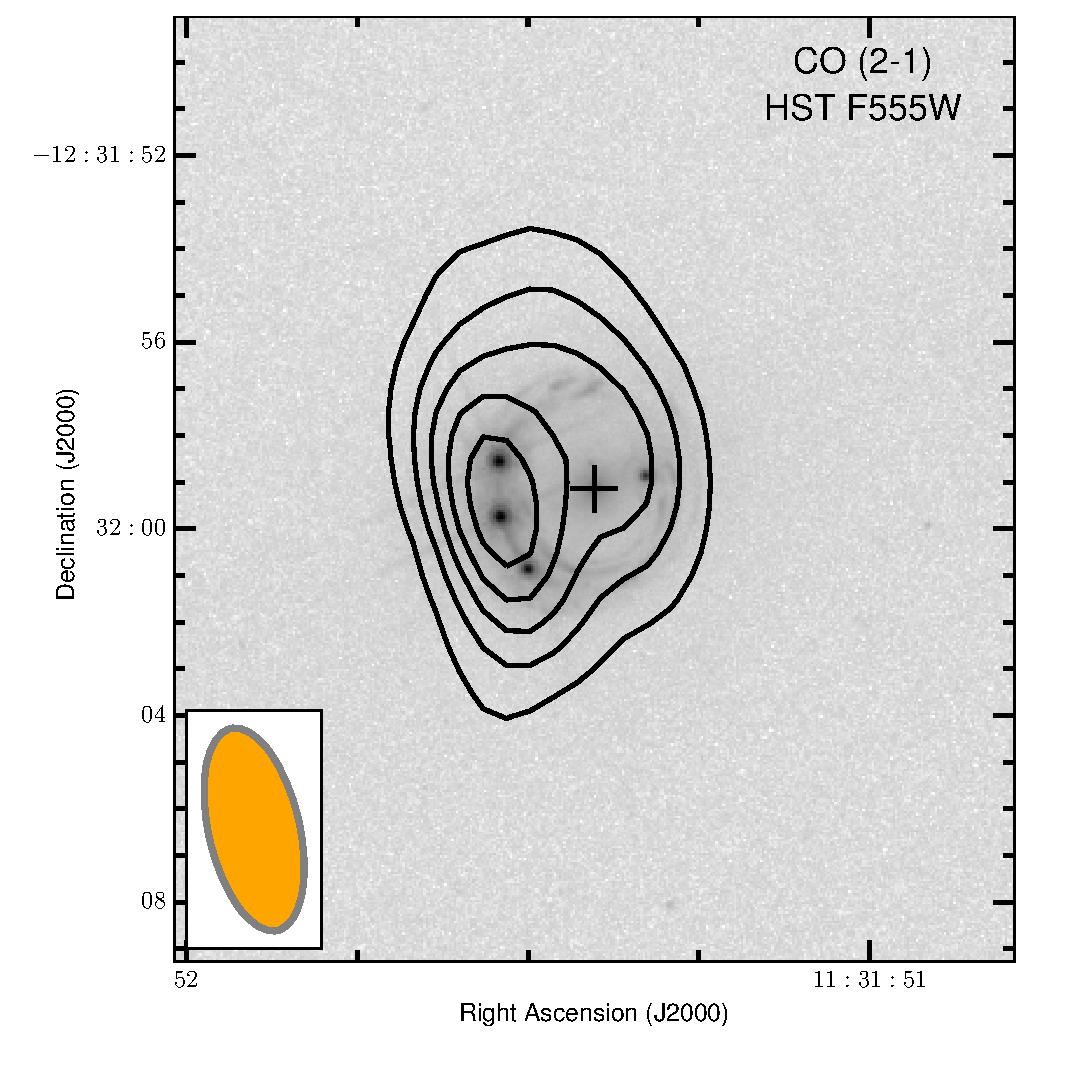
\includegraphics[scale=.3]{Fig/F555WCO21_mom0_single_invertedgray}
\includegraphics[scale=0.23]{Fig/SpecCO21}
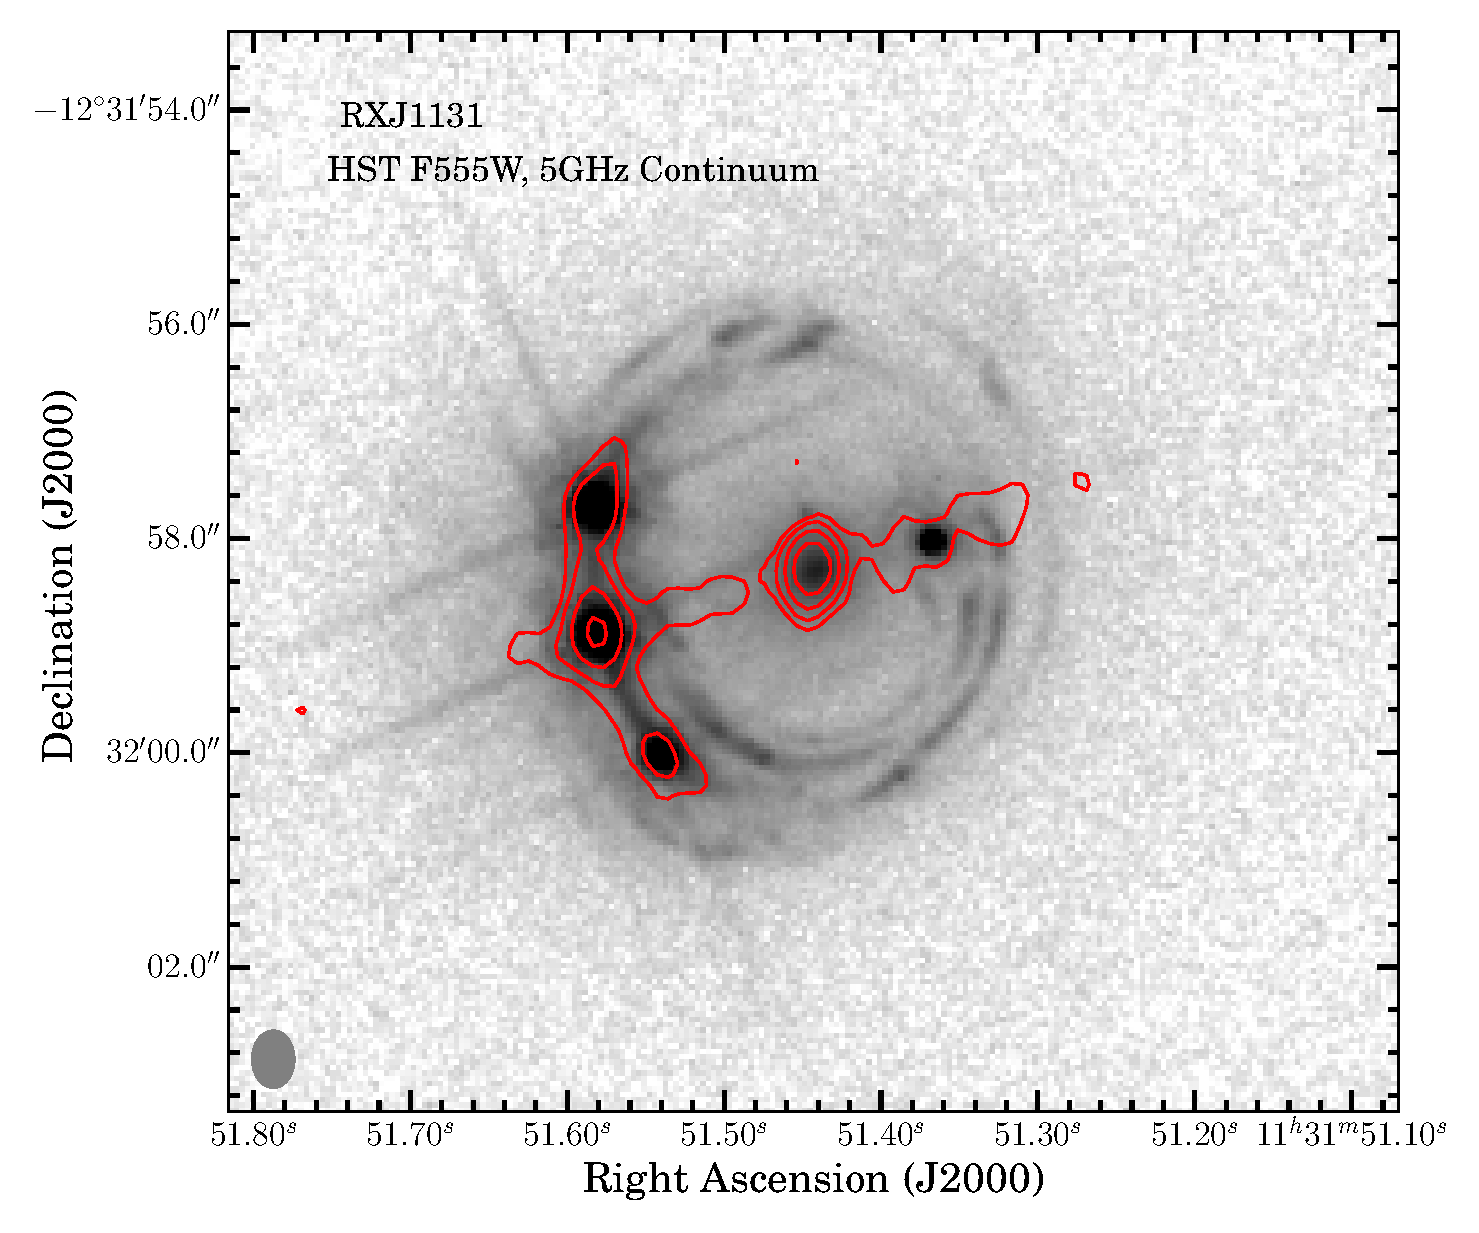
\includegraphics[scale=.2]{Fig/F555W_ContVLA}
\includegraphics[trim=0 0 0 30, clip, scale=0.36]{Fig/SED_mani} \vspace{-0.25em}
\caption{
{\bf Our target RXJ1131, a gas-rich, starbursting merger at $z$\,$>$\,0.6 with a well-sampled spectral energy distribution (SED) spanning rest-frame UV to radio.} 
{\em Top left:} Source-plane reconstruction of {\it HST} images shows the
emission from recent star-formation in this AGN host galaxy and
the presence of a nearby companion (\citealt{Claeskens06a}).
{\em Top right:} 
CO line emission overlaid on an {\it HST} image, which shows BLAH BLAH
that RXJ1131 is lensed into an Einstein ring of diameter $\sim$3.6".
{\em Middle left:}
Our recent study finds a large molecular gas reservoir of $M_{\rm gas}$\,$\gtrsim$\,10$^{10}$\Msun in RXJ1131 and 
confirmed the presence of its companion, with a gas mass ratio of 7:1 \citep{Leung17a}. 
{\em Middle right:}
We have previously detected radio continuum emission at 5\,GHz towards this target.
The proposed \obs will provide an additional constraint on the radio continuum at 1\,GHz.
{\em Bottom:} Our best-fit model to the well-sampled SED 
indicates a strong apparent far-IR radiation of \LFIR$>$4\E{12}\,\Lsun, corresponding to
an intense star formation rate of SFR\ssim120 \Msun yr\pmOne (lensing-corrected).
The large molecular gas reservoir, on-going star formation, and the high \LFIR together
are favourable for generating OHM, and thus RXJ1131 is an
ideal candidate for high-$z$ OHM search.
The proposed \obs together with our existing data acquired for this target will allow us to 
compare its (host) properties against those of local OHM hosts to better understand 
the physical environment that triggers OHM out to a look-back time of 6 Gyr.
\label{fig:hst}}
\end{figure}



\end{document}
